%!TEX root = SysSpec_ClockPendulumAnalyzer.tex
\section{Hardware Komponenten}
Um die Pendeldurchgänge der zu messenden Uhr erfassen, vergleichen und auswerten zu können, werden diverse Hardwarebausteine benötigt. In diesem Kapitel werden die Aufgabe und Entscheidungsgrundlagen beschrieben.
\subsection{IR-Sensoren}
	Alle in Frage kommenden Sensoren für die Ermittlung der Pendeldurchgänge basieren auf optischer Technologie, da Schallsensoren nicht genau genug sind oder zu nahe am Pendel platziert werden müsten. Mechanische Sensoren können aufgrund der physikalischen Effekte auf das Pendel verworfen werden.\\
	 Bei den optischen Sensoren stellt sich die Frage, ob der Sender und der Empfänger sich im gleichen Sensor befinden und ob ein Reflektor benötigt wird oder nicht.\\
	Aufgrund der unterschiedlichen Bauarten der Pendeluhren haben wir uns bezüglich für einen Sensortyp entschieden, welcher keinen Reflektor benötigt und bei dem Sender und Empfänger sehr nahe beieinander liegen. Auf diese Weise sind auch kleine Pendel messbar und es müssen keine Reflektoren angebracht und ausgerichtet werden.\\
	Aus Kostengründen und seiner kleinen Baugrösse haben wir uns für die Reflektions-Lichtschranke SFH9201 von Osram entschieden (Abbildung \ref{fig:SFH9201}).
	\begin{figure}[H]
        \centering
        \includegraphics[width=.5\textwidth]{reflexions-lichtschranke-sfh91019201-osram-1-st}
        \caption{Reflexlions-Lichtschranke Osram SFH9201 (Bildquelle: www.conrad.ch)}
        \label{fig:SFH9201}
    \end{figure}
	Der Sender befindet sich im kleineren, oberen Rechteck und der Empfänger im Unteren. Die detaillierten Eigenschaften können dem Datenblatt im Anhang, Seite <tbd> entnommen werden. Anbei die zentralen Eigenschaften:
	\begin{table}[H]
		\begin{tabular}{|p{11cm}|p{4cm}|}\hline
			Reaktionszeit auf Auslösung (Anstiegszeit): & 50$\mu{s}$ \\ \hline
			Bauteilhöhe:								& 4.2mm\\ \hline
			Bauteilbreite:								& 6.2mm inkl Anschlusspins\\ \hline
			Optimaler Arbeitsabstand:					& 1mm bis 5mm \\ \hline
		\end{tabular}
		\caption{Übersicht der Eigenschaften der Reflektions-Lichtschranke SFH9201}
		\label{tab:SFH9201}
	\end{table}
\subsection{GPS Modul}
	Ein GPS Modul wird benötigt um den Sekundentakt exakt zu synchronisieren und so keinere Ungenauigkeiten der Messfrequenz ausgleichen zu können. Weiter dient das GPS-Modul zur Ermittlung der aktuellen Absolut-Zeit.\\
	Die Positionsfunktion des GPS-Moduls wird nicht benötigt und implementiert. Gemeinsam mit der externen Real-Time Clock ist unsere Wahl beim GPS-Modul auf ein Modell aus der Feather-Wing Familie von Adafruit gefallen (Abbildung \ref{fig:GPS3133}). Ausschlaggebend dafür sind modularität, Kosten und Funktionsumfang. Das GPS -Modul bietet direkt einen 1-Sekunden-Puls über den FIX-Pin, wenn keine GPS-Verbindung besteht sowie über den PPS-Pin bei vorhandener Verbindung. Somit ist ein Referenzsignal auch bei unterbrochener Verbindung verfügbar, wenn auch nicht mit der gleichen Genauigkeit. Die GPS-Zeitgenauigkeit ist im Datenblatt von Adafruit, Angang ab Seite <tbd> nicht angegeben, die GPS-Genauigkeit bezüglich des Sekundenpulses liegt im Bereich von <40ns (gpstime.com). Die Genauigkeit des Sekunden-Pulses im Offline-Modus ist nicht verfügbar, da nicht im Datenblatt enthalten. Für eine präzise Messung ist somit eine GPS-Verbindung Pflicht. Für funktionale Systemtests ohne Berücksichtigung der Messgenauigkeit ist der Offline-Sekundenpuls ausreichend.
		\begin{figure}[H]
        	\centering
        	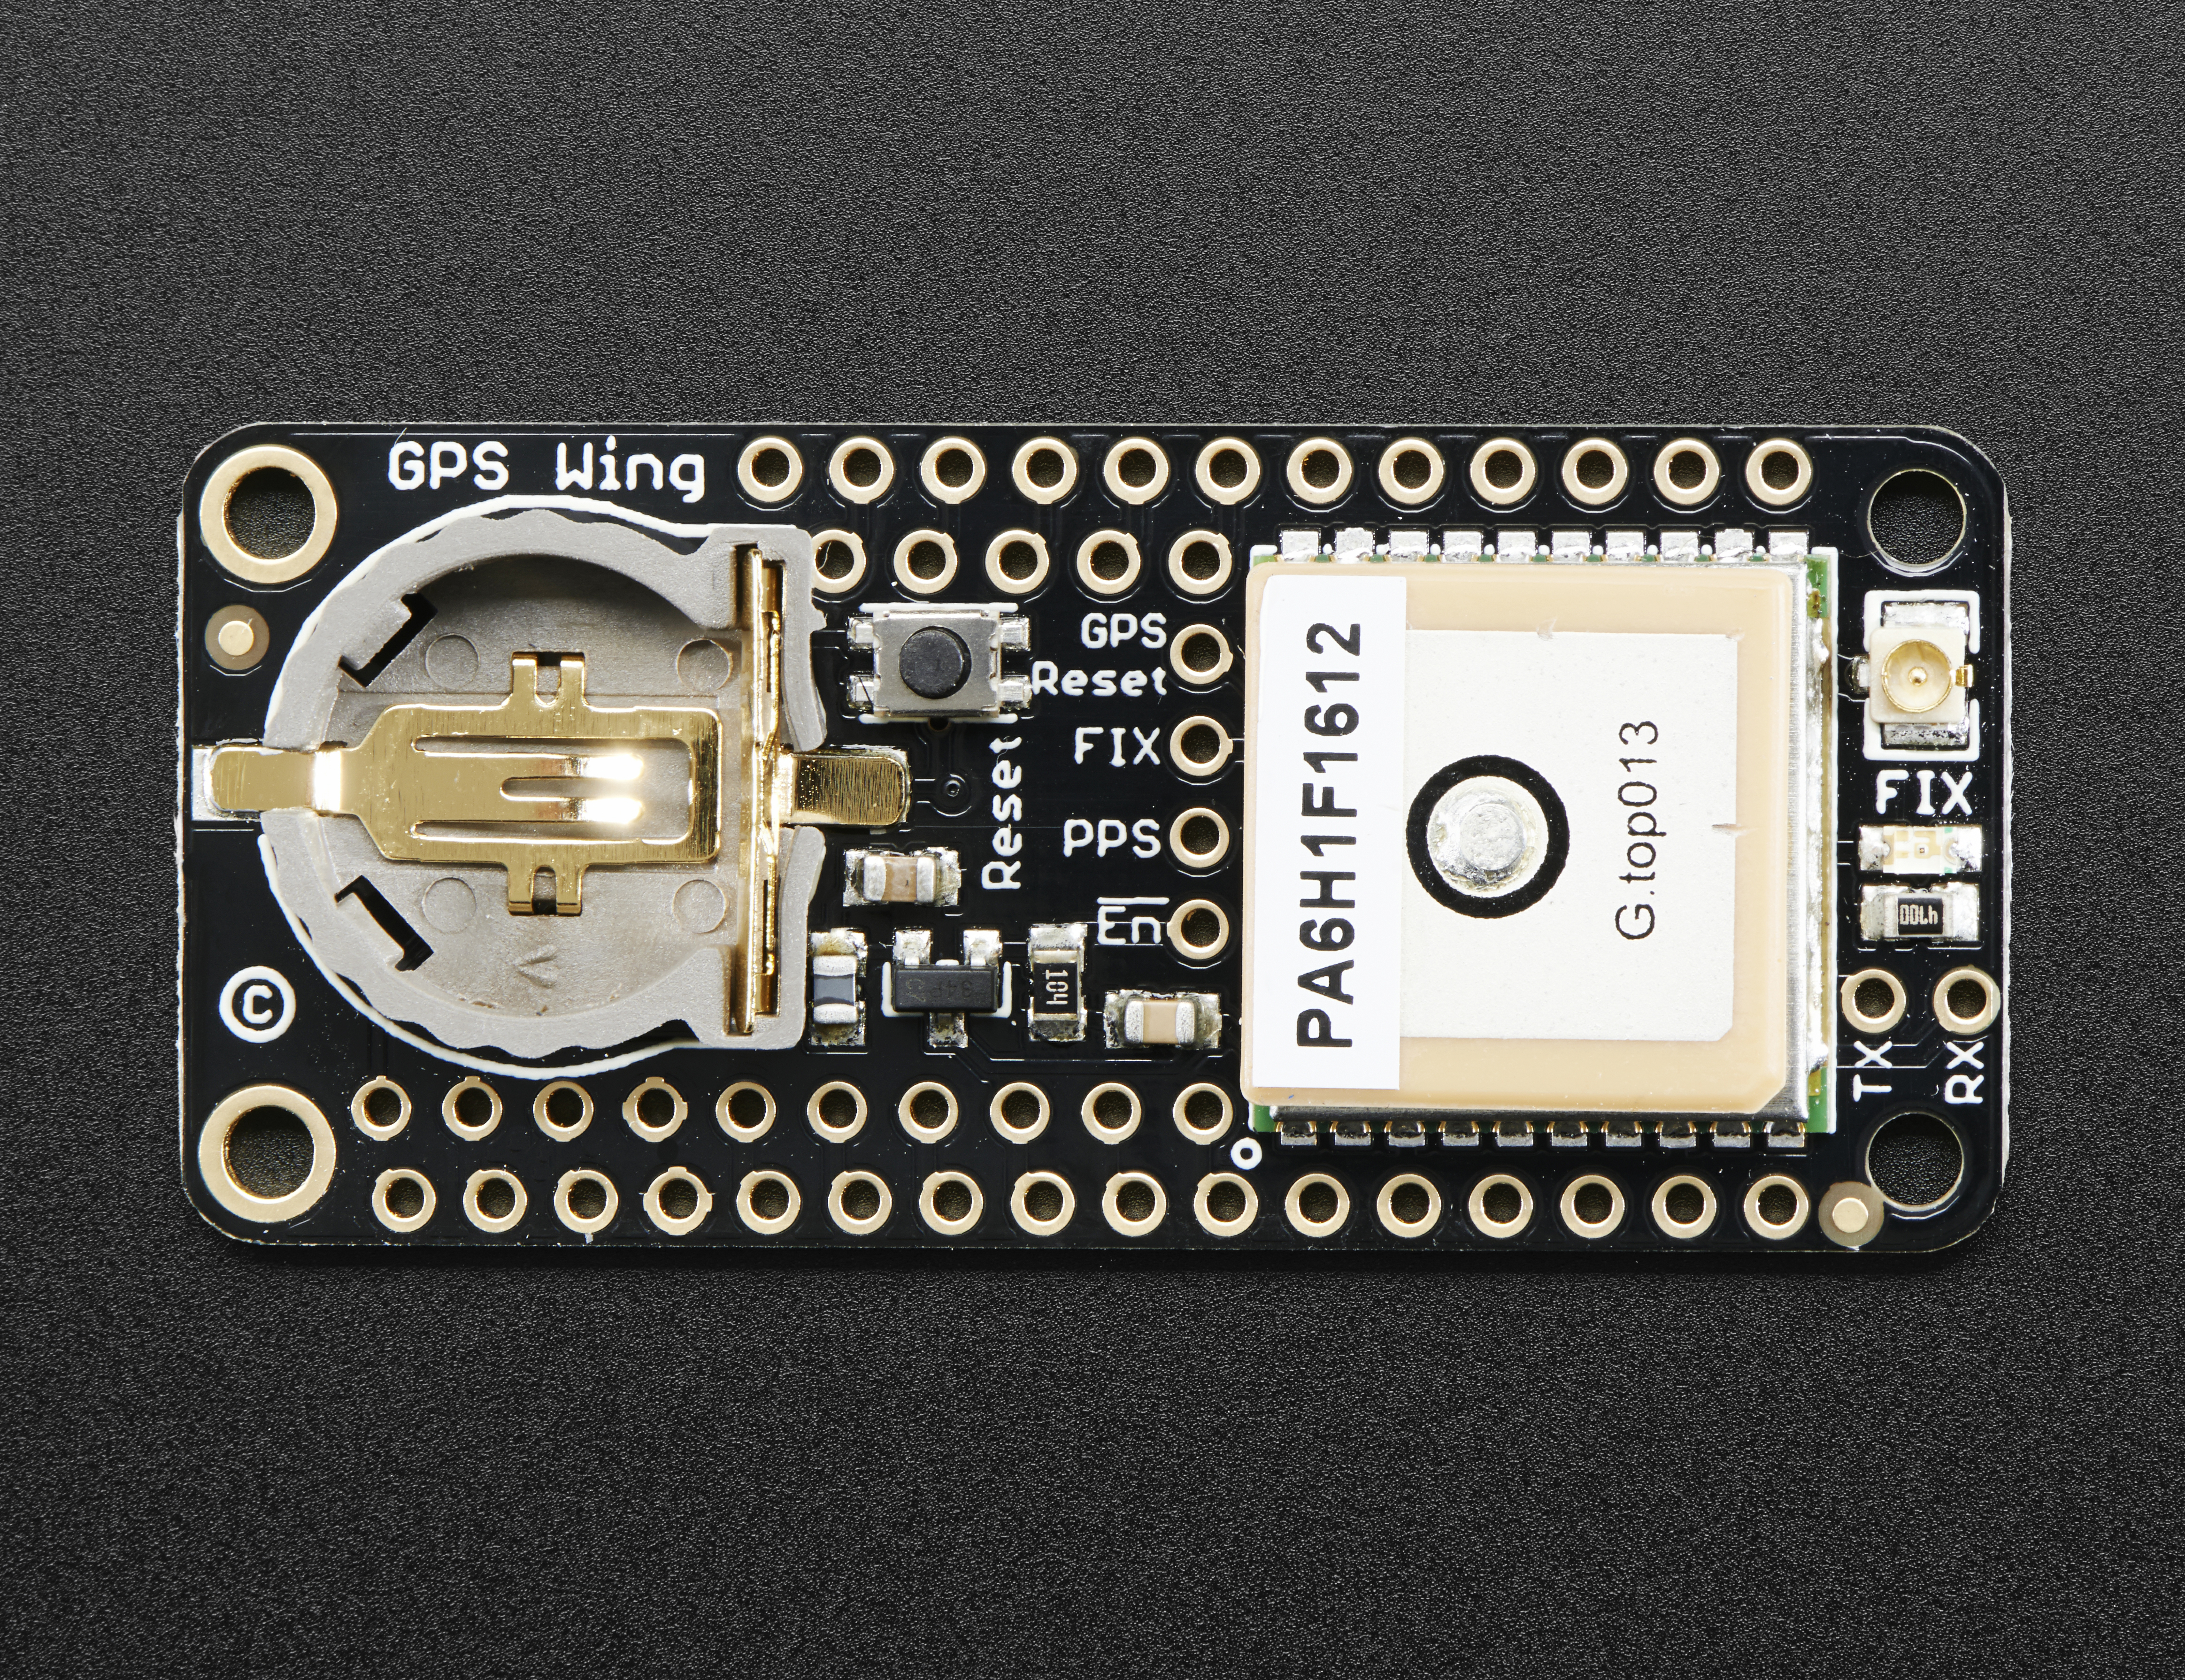
\includegraphics[width=.5\textwidth]{gps_3133_top}
        	\caption{GPS-Modul Draufsicht mit den Pins PPS und FIX (Bildquelle: learn.adafruit.com)}
        	\label{fig:GPS3133}
    	\end{figure}
	Zur Nutzung des GPS Moduls zum Setzen der Systemzeit kann das GPS-Modul über UART RS232 an den RX-TX Pins ansgeschlossen und angesprochen werden.    	
\subsection{Real Time Clock}
	Die Real-Time Clock (RTC) kann als externer Frequenzgeber verwendet werden, da sie über ein 32KHz signal verfügt, welches eine Abweichung von +/- 2 ppm\footnote{Parts Per Million} auf ein \textbf{TODO: exakte Zeiteinheit für die Toleranz einfügen} verspricht.\\
	Weiter verfügt die RTC über die Möglichkeit, dem Raspberry PI die Absolutzeit zu vermitteln, wenn z.B. keine Netwerkverbindung besteht oder kein NTP\footnote{Network Time Protocol} verfügbar ist.
\subsection{Hardware Counter}
%!TEX root = SysSpec_ClockPendulumAnalyzer.tex
\subsection{Raspberry Pi}
Die ganze Software wird mittels C++ auf einem Raspberry Pi Version 3 (kurz RPi3) ausgeführt.

\subsubsection{Entscheidungsgrundlage}
Für die Umsetzung auf Computerebene wurde entschieden kein Realtime OS zu verwenden. Das führte dazu, dass eine der möglichen Lösungen auf das Raspberry Pi fiel. Das Raspberry bietet eine weitverbreitete und aktive Community. Dadurch kann bei Problemen leicht auf gute Lösungsvorschläge zugegriffen werden.\\
Um mit der Hardware auf einem guten Stand zu sein, wurde die neuste Version 3 des Raspberry Pi gewählt.

\subsubsection{Betriebssystem und Software}
Für das Betriebssystem wird ein extrem leicht gewichtetes OS verwendet. Dies verhindert dass ungewünschte daemons oder andere Programme den Betrieb verlangsamen. Es wird daher nur das allernötigste installiert. In der untenstehenden Auflistung sind alle zusätzlich installierten Programme aufgelistet. 

\begin{table}[h]
    \begin{tabular}{ll}
        ArchlinuxARM & OS für Raspberry Pi\\
        i2c-tools 3.1.2-1 & i2c tool set für Linux\\
        libconfig & C/C++ Konfiguration Datei Bibliothek\\
        libbcm2835 & Broadcom BCM 2835 c Bibliothek für Raspberry Pi\\
    \end{tabular}
    \caption{installierte Software auf dem RPi3}
\end{table}

\noindent Das Betriebssystem wird mit einem Benutzer und möglichem SSH Zugriff eingerichtet. Um per SSH auf das Raspberry zugreifen zu können muss der Host im Netzwerk 192.168.192.0/24 sein.
\begin{table}[h]
    \begin{tabular}{ll}
        Benutzer: & clockpendulum \\
        Passwort: & cpa\_admin \\
        IP: & 192.168.192.75 \\
    \end{tabular}
    \caption{Daten für den Zugriff auf das RPi3}
\end{table}
%user: clockpendulum
%pw: cpa_admin